% Choose one to switch between slides and handout
%\documentclass[]{beamer}
\documentclass[handout]{beamer}

% Video Meta Data
\title{Bitcoin, Blockchain and Cryptoassets}
\subtitle{Transaction Examples}
\author{Prof. Dr. Fabian Schär}
\institute{University of Basel}

% Config File
% Packages
\usepackage[utf8]{inputenc}
\usepackage{hyperref}
\usepackage{gitinfo2}
\usepackage{tikz}
\usepackage{amsmath}
\usepackage{bibentry}
\usepackage{xcolor}
\usepackage{colortbl} % Add colour to LaTeX tables
\usepackage{caption}
\usepackage[export]{adjustbox}
\usepackage{pgfplots} \pgfplotsset{compat = 1.17}

% Color Options
\definecolor{highlight}{rgb}{0.65,0.84,0.82}
\definecolor{focus}{rgb}{0.72, 0, 0}

% Beamer Template Options
\beamertemplatenavigationsymbolsempty
\setbeamertemplate{footline}[frame number]
\setbeamercolor{structure}{fg=black}
\setbeamercolor{footline}{fg=black}
\setbeamercolor{title}{fg=black}
\setbeamercolor{frametitle}{fg=black}
\setbeamercolor{item}{fg=black}
\setbeamercolor{}{fg=black}
\setbeamercolor{bibliography item}{fg=black}
\setbeamercolor*{bibliography entry title}{fg=black}
\setbeamertemplate{items}[square]
\setbeamertemplate{enumerate items}[default]
\captionsetup[figure]{labelfont={color=black},font={color=black}}
\captionsetup[table]{labelfont={color=black},font={color=black}}

\setbeamertemplate{bibliography item}{\insertbiblabel}

% Link Icon Command
\newcommand{\link}{%
    \tikz[x=1.2ex, y=1.2ex, baseline=-0.05ex]{%
        \begin{scope}[x=1ex, y=1ex]
            \clip (-0.1,-0.1)
                --++ (-0, 1.2)
                --++ (0.6, 0)
                --++ (0, -0.6)
                --++ (0.6, 0)
                --++ (0, -1);
            \path[draw,
                line width = 0.5,
                rounded corners=0.5]
                (0,0) rectangle (1,1);
        \end{scope}
        \path[draw, line width = 0.5] (0.5, 0.5)
            -- (1, 1);
        \path[draw, line width = 0.5] (0.6, 1)
            -- (1, 1) -- (1, 0.6);
        }
    }

% Read Git Data from Github Actions Workflow
% Defaults to gitinfo2 for local builds
\IfFileExists{gitInfo.txt}
	{\input{gitInfo.txt}}
	{
		\newcommand{\gitRelease}{(Local Release)}
		\newcommand{\gitSHA}{\gitHash}
		\newcommand{\gitDate}{\gitAuthorIsoDate}
	}

% Custom Titlepage
\defbeamertemplate*{title page}{customized}[1][]
{
  \vspace{-0cm}\hfill
\includegraphics[width=2.5cm]{../config/logo_cif}
  
\includegraphics[width=1.9cm]{../config/seal_wwz}
  \\ \vspace{2em}
  \usebeamerfont{title}\textbf{\inserttitle}\par
  \usebeamerfont{title}\usebeamercolor[fg]{title}\insertsubtitle\par  \vspace{1.5em}
  \small\usebeamerfont{author}\insertauthor\par
  \usebeamerfont{author}\insertinstitute\par \vspace{2em}
  \usebeamercolor[fg]{titlegraphic}\inserttitlegraphic
    \tiny \noindent \texttt{Release Ver.: \gitRelease}\\ 
    \texttt{Version Hash: \gitSHA}\\
    \texttt{Version Date: \gitDate}\\ \vspace{1em}
  \link \href{https://github.com/cifunibas/Bitcoin-Blockchain-Cryptoassets/blob/main/slides/intro.pdf}
  {Get most recent version}\\
  \link \href{https://github.com/cifunibas/Bitcoin-Blockchain-Cryptoassets/blob/main/slides/intro.pdf}
  {Watch video lecture}\\ \vspace{1em}
  License: \texttt{Creative Commons Attribution-NonCommercial-ShareAlike 4.0 International}\\\vspace{2em}
  
\includegraphics[width = 1.2cm]{../config/license}
}

% tikzlibraries
\usetikzlibrary{decorations.pathreplacing}
\usetikzlibrary{decorations.markings}
\usetikzlibrary{positioning}

%caption font
\captionsetup{font=footnotesize}


%%%%%%%%%%%%%%%%%%%%%%%%%%%%%%%%%%%%%%%%%%%%%%
%%%%%%%%%%%%%%%%%%%%%%%%%%%%%%%%%%%%%%%%%%%%%%
\begin{document}

\thispagestyle{empty}
\begin{frame}[noframenumbering]
	\titlepage
\end{frame}

%%%
\begin{frame}{Prerequisites}
	\begin{itemize}
		\item<1->{Hexadecimal values (Base 16)}
		\item<2->{Endianness:}
			\begin{itemize}
				\item<2->{1 in big-endian: 00000001}
				\item<3->{1 in little-endian: 01000000}
			\end{itemize}
		\item<4->{Hash functions}
		\item<5->{ECDSA}\\
	\end{itemize}
\end{frame}
%%%	


%%%
\begin{frame}{Pay-to-Public-Key}
	\href{https://blockstream.info/tx/f4184fc596403b9d638783cf57adfe4c75c605f6356fbc91338530e9831e9e16}{\link The first Bitcoin transaction:}
	\begin{figure}
		\begin{tikzpicture}
	\node (Satoshi) at (-3,0)[label=below: Satoshi Nakamoto] {
\includegraphics[height = 0.2\textheight]{../assets/images/agents/handing_money_right.png}};
	\node (Hal) at (3, 0)[label=below: Hal Finney] {
\includegraphics[height = 0.2\textheight]{../assets/images/agents/reaching_left.png}};
	
	\uncover<2->{
		\draw[->, ultra thick] (Satoshi.east) -- (Hal.west) node[midway, above] {10 BTC};
	}
	
	\uncover<3->{
		\node (pubKey1) at (-3, -3.5) {\scriptsize{$K_{pub,Satoshi} = $
		\begin{tabular}{l} \texttt{04}\\
			\texttt{\color{focus}{11db93e1dcdb8a01}}\\
			\texttt{\color{focus}{6b49840f8c53bc1e}}\\
			\texttt{\color{focus}{b68a382e97b1482e}}\\
			\texttt{\color{focus}{cad7b148a6909a5c}}\\
			\texttt{\color{highlight}{b2e0eaddfb84ccf9}}\\
			\texttt{\color{highlight}{744464f82e160bfa}}\\
			\texttt{\color{highlight}{9b8b64f9d4c03f99}}\\
			\texttt{\color{highlight}{9b8643f656b412a3}}\\
		\end{tabular}}};
	}
	
	\uncover<3->{
		\node (pubKey1) at (3, -3.5) {\scriptsize{$K_{pub,Hal} = $
		\begin{tabular}{l} \texttt{04}\\
			\texttt{\color{focus}{ae1a62fe09c5f51b}}\\
			\texttt{\color{focus}{13905f07f06b99a2}}\\
			\texttt{\color{focus}{f7159b2225f374cd}}\\
			\texttt{\color{focus}{378d71302fa28414}}\\
			\texttt{\color{highlight}{e7aab37397f554a7}}\\
			\texttt{\color{highlight}{df5f142c21c1b730}}\\
			\texttt{\color{highlight}{3b8a0626f1baded5}}\\
			\texttt{\color{highlight}{c72a704f7e6cd84c}}
		\end{tabular}}};
	}
	
\end{tikzpicture}
	\end{figure}
\end{frame}
%%%

%%%
\begin{frame}{Transaction Inputs}
	\begin{figure}
		 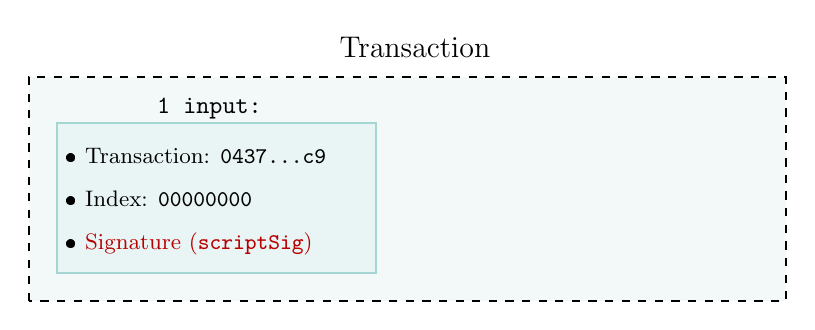
\begin{tikzpicture}[scale=0.9, every node/.style={scale=0.9}]
    
        \filldraw[yshift=-0.05cm, xshift=0.1cm,color = highlight!15, thick, draw=black, dashed] (-4,-4) rectangle ++(304pt,90pt) ;
    
        \filldraw[yshift=-0.05cm, xshift=0.1cm,color = highlight!25, thick, draw=highlight] (-3.6,-3.6) rectangle ++(128pt,60pt) ;
     
    \draw[color=black] plot (-1.35,-1.6) node[above] {\texttt{1 input:}};
    \draw[color=black] plot (-3.5,-2) node[right] {\small{\textbullet{} Transaction: \texttt{0437...c9}}};
    \draw[color=black] plot (-3.5,-2.6)   node[right] {\small{\textbullet{} Index: \texttt{00000000}}};
    \draw[color=black] plot (-3.5,-3.25)   node[right] {\small{\textbullet{} \textcolor{focus}{Signature (\texttt{scriptSig})}}};
    \draw[color=black] plot (1.55,-0.2) node [below]
    {\large{{Transaction}}};
    
\end{tikzpicture}
	\end{figure}
	\uncover<2->{
		\scriptsize
			\begin{tabular}{ll}
				\texttt{scriptPubKey} from the previous transaction: & \\
				\textcolor{black!50}{\texttt{OP\_PUSHBYTES\_65:}} & \textcolor{black!50}{\texttt{41}}\\
				Uncompressed public key: & \texttt{04}\\
				Public key: & \texttt{11db93e1dcdb8a016b49840f8c53bc1e}\\
				 & \texttt{b68a382e97b1482ecad7b148a6909a5c}\\
				 & \texttt{b2e0eaddfb84ccf9744464f82e160bfa}\\
				 & \texttt{9b8b64f9d4c03f999b8643f656b412a3}\\
				\textcolor{black!50}{\texttt{OP\_CHECKSIG:}} & \textcolor{black!50}{\texttt{ac}}
			\end{tabular}
	}
	\vspace{0.5em}\\
	\small
	\uncover<3->{$\rightarrow$ If you know the private key to \texttt{11db...a3} you can spend the UTXO \phantom{$\rightarrow$} of 50 BTC.}
\end{frame}
%%%

%%%
\begin{frame}{Transaction Outputs}
	\begin{figure}
		 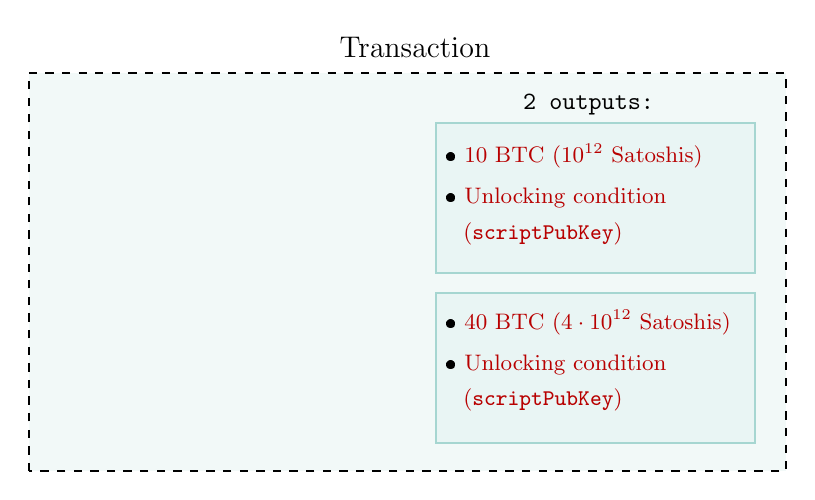
\begin{tikzpicture}[scale=0.9, every node/.style={scale=0.9}]
    
        \filldraw[yshift=-0.05cm, xshift=0.1cm,color = highlight!15, thick, draw=black, dashed] (-4,-6.4) rectangle ++(304pt,160pt) ;
        
    \draw[color=black] plot (1.55,-0.2) node [below]
    {\large{{Transaction}}};

    
        \filldraw[yshift=-0.05cm, xshift=0.1cm,color = highlight!25, thick, draw=highlight] (1.75,-3.6) rectangle ++(128pt,60pt) ;
    
    \draw[color=black] plot (4,-1.55)   node[above] {\texttt{2 outputs:}};
    \draw[color=black] plot (1.85,-2)   node[right] {\small{\textbullet{} \textcolor{focus}{10 BTC ($10^{12}$ Satoshis)}}};
    \draw[color=black] plot (1.85,-2.6)   node[right] {\small{\textbullet{} \textcolor{focus}{Unlocking condition}}};
    \draw[color=black] plot (2,-3.1)   node[right] {\small{ \textcolor{focus}{(\texttt{scriptPubKey})}}};

	\filldraw[yshift=-0.05cm, xshift=0.1cm,color = highlight!25, thick, draw=highlight] (1.75,-6) rectangle ++(128pt,60pt) ;

    \draw[color=black] plot (1.85,-4.35)   node[right] {\small{\textbullet{} \textcolor{focus}{40 BTC ($4 \cdot 10^{12}$ Satoshis)}}};
    \draw[color=black] plot (1.85,-4.95)   node[right] {\small{\textbullet{} \textcolor{focus}{Unlocking condition}}};
    \draw[color=black] plot (2,-5.45)   node[right] {\small{ \textcolor{focus}{(\texttt{scriptPubKey})}}};

\end{tikzpicture}
	\end{figure}
\end{frame}

\begin{frame}{Transaction Outputs}
	\scriptsize
	\textbf{First output:}\\
	\begin{tabular}{ll}
	10 BTC & = 1,000,000,000 Satoshis\\
	\uncover<2->{& = \texttt{00ca9a3b00000000} as little-endian integer}\\
	\uncover<3->{\texttt{scriptPubKey:} & \\
		\textcolor{black!50}{\texttt{OP\_PUSHBYTES\_65:}} & \textcolor{black!50}{\texttt{41}}\\
		Uncompressed public key: & \texttt{04}\\
		Public key: & \texttt{ae1a62fe09c5f51b13905f07f06b99a2}\\
		 & \texttt{f7159b2225f374cd378d71302fa28414}\\
		 & \texttt{e7aab37397f554a7df5f142c21c1b730}\\
		 & \texttt{3b8a0626f1baded5c72a704f7e6cd84c}\\
		\textcolor{black!50}{\texttt{OP\_CHECKSIG:}} & \textcolor{black!50}{\texttt{ac}}
	}
	\end{tabular}
	\vspace{1em}\\
	\textbf{Second output (''change"):}\\
	\begin{tabular}{ll}
	40 BTC & = 4,000,000,000 Satoshis\\
	\uncover<2->{& = \texttt{00286bee00000000} as little-endian integer}\\
	\uncover<3->{\texttt{scriptPubKey:} & \\
		\textcolor{black!50}{\texttt{OP\_PUSHBYTES\_65:}} & \textcolor{black!50}{\texttt{41}}\\
		Uncompressed public key: & \texttt{04}\\
		Public key: & \texttt{11db93e1dcdb8a016b49840f8c53bc1e}\\
		 & \texttt{b68a382e97b1482ecad7b148a6909a5c}\\
		 & \texttt{b2e0eaddfb84ccf9744464f82e160bfa}\\
		 & \texttt{9b8b64f9d4c03f999b8643f656b412a3}\\
		\textcolor{black!50}{\texttt{OP\_CHECKSIG:}} & \textcolor{black!50}{\texttt{ac}}
	}
	\end{tabular}

\end{frame}

\begin{frame}{Transaction Inputs and Outputs}
	\begin{figure}
		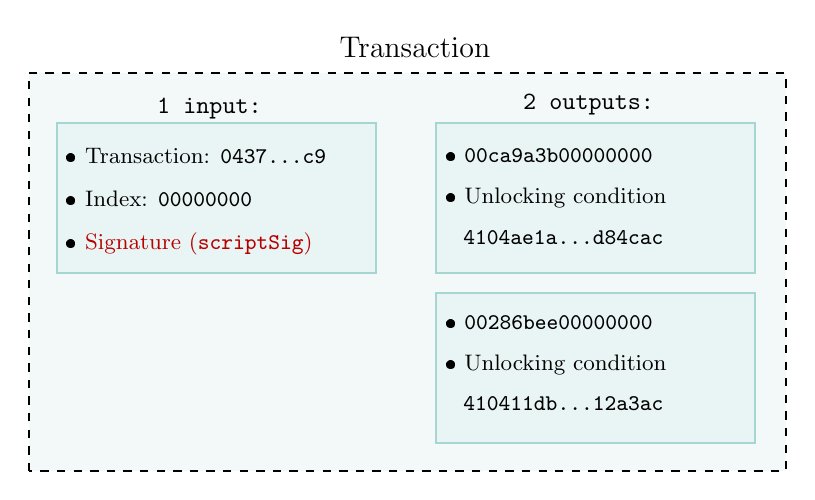
\begin{tikzpicture}[scale=0.9, every node/.style={scale=0.9}]
    
        \filldraw[yshift=-0.05cm, xshift=0.1cm,color = highlight!15, thick, draw=black, dashed] (-4,-6.4) rectangle ++(304pt,160pt) ;
        
    \draw[color=black] plot (1.55,-0.2) node [below]
    {\large{{Transaction}}};

    
    \filldraw[yshift=-0.05cm, xshift=0.1cm,color = highlight!25, thick, draw=highlight] (1.75,-3.6) rectangle ++(128pt,60pt) ;
    
    \filldraw[yshift=-0.05cm, xshift=0.1cm,color = highlight!25, thick, draw=highlight] (-3.6,-3.6) rectangle ++(128pt,60pt) ;
     
    \draw[color=black] plot (-1.35,-1.6) node[above] {\texttt{1 input:}};
    \draw[color=black] plot (-3.5,-2) node[right] {\small{\textbullet{} Transaction: \texttt{0437...c9}}};
    \draw[color=black] plot (-3.5,-2.6)   node[right] {\small{\textbullet{} Index: \texttt{00000000}}};
    \draw[color=black] plot (-3.5,-3.25)   node[right] {\small{\textbullet{} \textcolor{focus}{Signature (\texttt{scriptSig})}}};

    
    \draw[color=black] plot (4,-1.55)   node[above] {\texttt{2 outputs:}};
    \draw[color=black] plot (1.85,-2)   node[right] {\small{\textbullet{} \texttt{00ca9a3b00000000}}};
    \draw[color=black] plot (1.85,-2.6)   node[right] {\small{\textbullet{} Unlocking condition}};
    \draw[color=black] plot (2,-3.15)   node[right] {\small{ \texttt{4104ae1a...d84cac}}};

	\filldraw[yshift=-0.05cm, xshift=0.1cm,color = highlight!25, thick, draw=highlight] (1.75,-6) rectangle ++(128pt,60pt) ;

    \draw[color=black] plot (1.85,-4.35)   node[right] {\small{\textbullet{} \texttt{00286bee00000000}}};
    \draw[color=black] plot (1.85,-4.95)   node[right] {\small{\textbullet{} Unlocking condition}};
    \draw[color=black] plot (2,-5.5)   node[right] {\small{ \texttt{410411db...12a3ac}}};

\end{tikzpicture}	
	\end{figure}

\end{frame}


%%%
%\begin{frame}{Transaction Hash}
%\begin{itemize}
%\item Transaction Hash: \\
%{\scriptsize \texttt{f4184fc596403b9d638783cf57adfe4c75c605f6356fbc91338530e9831e9e16}}
%\item SHA256(SHA256(Raw TRX Data)) $\rightarrow$ TRX Hash
%\end{itemize}
%\end{frame}
%%%	

%%%
\begin{frame}{Raw Transaction Data (Outputs)}
\begin{scriptsize}
\texttt{\textcolor{black!30}{0100000001c997a5e56e104102fa209c6a852dd90660a20b2d9c352423edce25857fcd3704
000000004847304402204e45e16932b8af514961a1d3a1a25fdf3f4f7732e9d624c6c61548
ab5fb8cd410220181522ec8eca07de4860a4acdd12909d831cc56cbbac4622082221a8768d
1d0901ffffffff}{\alert<2>{02}\alert<3>{00ca9a3b00000000}\alert<4>{43}\alert<5>{41}\alert<6>{04}\alert<7>{ae1a62fe09c5f51b13905f07f06b99a2f715
9b2225f374cd378d71302fa28414e7aab37397f554a7df5f142c21c1b7303b8a0626f1bade
d5c72a704f7e6cd84c}\alert<8>{ac}\alert<9>{00286bee00000000}\alert<10>{43}\alert<11>{41}\alert<12>{04}\alert<13>{11db93e1dcdb8a016b49840f8c53bc1e
b68a382e97b1482ecad7b148a6909a5cb2e0eaddfb84ccf9744464f82e160bfa9b8b64f9d4
c03f999b8643f656b412a3}\alert<14>{ac}}\textcolor{black!30}{00000000}}
\end{scriptsize}
\vspace{1em}
\scriptsize \\
\textbf{The outputs consists of:}\\
\begin{columns}[T]
\column{0.5\textwidth}
\begin{itemize}
	\item \alert<2>{2 outputs: \texttt{02}}
	\item \alert<3>{10 BTC: \texttt{00ca9a3b00000000}}
	\item \alert<4>{\texttt{scriptPubKey} is 67 bytes long: \texttt{43}}
	\item \alert<5>{Public key is 65 bytes long: \texttt{41}}
	\item \alert<6>{Uncompressed public key: \texttt{04}}
	\item \alert<7>{Public key: \texttt{ae1a...d84c}}
	\item \textcolor{black!50}{\alert<8>{\texttt{OP\_CHECKSIG}: \texttt{ac}}}
\end{itemize}
\column{0.5\textwidth}
\begin{itemize}
	\item \alert<9>{40 BTC (''change"): \texttt{00286bee00000000}}
	\item \alert<10>{\texttt{scriptPubKey} is 67 bytes long: \texttt{43}}
	\item \alert<11>{Public key is 65 bytes long: \texttt{41}}
	\item \alert<12>{Uncompressed public key: \texttt{04}}
	\item \alert<13>{Public key: \texttt{11db...12a3}}
	\item \textcolor{black!50}{\alert<14>{\texttt{OP\_CHECKSIG}: \texttt{ac}}}
\end{itemize}
\end{columns}

\end{frame}
%%%

%%%
\begin{frame}{Raw Transaction Data (Input)}
\begin{scriptsize}
\texttt{\textcolor{black!30}{01000000}{\alert<2>{01}\alert<3>{c997a5e56e104102fa209c6a852dd90660a20b2d9c352423edce25857fcd3704}
\alert<4>{00000000}}\textcolor{black!30}{4847304402204e45e16932b8af514961a1d3a1a25fdf3f4f7732e9d624c6c61548
ab5fb8cd410220181522ec8eca07de4860a4acdd12909d831cc56cbbac4622082221a8768d
1d0901ffffffff0200ca9a3b00000000434104ae1a62fe09c5f51b13905f07f06b99a2f715
9b2225f374cd378d71302fa28414e7aab37397f554a7df5f142c21c1b7303b8a0626f1bade
d5c72a704f7e6cd84cac00286bee0000000043410411db93e1dcdb8a016b49840f8c53bc1e
b68a382e97b1482ecad7b148a6909a5cb2e0eaddfb84ccf9744464f82e160bfa9b8b64f9d4
c03f999b8643f656b412a3ac00000000}}
\end{scriptsize}
\vspace{1em}
\scriptsize \\
\textbf{The input consists of:}\\
\begin{itemize}
	\item \alert<2>{1 input: \texttt{01}}
	\item \alert<3>{Previous transaction in reverse byte order: \texttt{c997a5e56e104102fa209c6a852dd90660a20b2d9c352423edce25857fcd3704}}
	\item \alert<4>{Index of the output within the previous transaction as little-endian integer: \texttt{00000000}}
\end{itemize}
\end{frame}
%%%


%%%
\begin{frame}{Raw Transaction Data (Signature)}
	\begin{scriptsize}
\texttt{\textcolor{black!30}{0100000001c997a5e56e104102fa209c6a852dd90660a20b2d9c352423edce25857fcd3704
00000000}{\alert<2>{48}\alert<3>{47}\alert<4>{30}\alert<5>{44}\alert<6>{02}\alert<7>{20}\alert<8>{4e45e16932b8af514961a1d3a1a25fdf3f4f7732e9d624c6c61548
ab5fb8cd41}\alert<9>{02}\alert<10>{20}\alert<11>{181522ec8eca07de4860a4acdd12909d831cc56cbbac4622082221a8768d
1d09}\alert<12>{01}}\textcolor{black!30}{ffffffff0200ca9a3b00000000434104ae1a62fe09c5f51b13905f07f06b99a2f715
9b2225f374cd378d71302fa28414e7aab37397f554a7df5f142c21c1b7303b8a0626f1bade
d5c72a704f7e6cd84cac00286bee0000000043410411db93e1dcdb8a016b49840f8c53bc1e
b68a382e97b1482ecad7b148a6909a5cb2e0eaddfb84ccf9744464f82e160bfa9b8b64f9d4
c03f999b8643f656b412a3ac00000000}}
\end{scriptsize}
\vspace{1em}
\scriptsize \\
\textbf{The signature consists of:}\\
\begin{columns}[T]
\column{0.5\textwidth}
\begin{itemize}
	\item \alert<2>{72 byte long \texttt{scriptSig}: \texttt{48}}
	\item \alert<3>{71 byte long signature: \texttt{47}}
	\item \alert<4>{DER sequence follows: \texttt{30}}
	\item \alert<5>{68 bytes long: \texttt{44}}
	\item \alert<6>{An integer follows: \texttt{02}}
	\item \alert<7>{The integer is 32 bytes long: \texttt{20}}
	\item \alert<8>{$r$ from the ECDSA signature: 	\texttt{4e45e16932b8af514961a1d3a1a25fdf\\3f4f7732e9d624c6c61548ab5fb8cd41}}
\end{itemize}
\column{0.5\textwidth}
\begin{itemize}
	\item \alert<9>{An integer follows: \texttt{02}}
	\item \alert<10>{The integer is 32 bytes long: \texttt{20}}
	\item \alert<11>{$s$ from the ECDSA signature: \texttt{181522ec8eca07de4860a4acdd12909d\\831cc56cbbac4622082221a8768d1d09}}
	\item \alert<12>{\texttt{SIGHASH\_ALL}: \texttt{01}}
\end{itemize}
\end{columns}
\vspace{1.5em}
\href{https://github.com/cifunibas/Bitcoin-Blockchain-Cryptoassets/blob/main/assets/scripts/satoshi_transaction.py}{\link Python script for the verification}
\end{frame}
%%%

%%%
\begin{frame}{Raw Transaction Data (Additional Data)}
\begin{scriptsize}
\texttt{\alert<2>{01000000}\textcolor{black!30}{01c997a5e56e104102fa209c6a852dd90660a20b2d9c352423edce25857fcd3704
000000004847304402204e45e16932b8af514961a1d3a1a25fdf3f4f7732e9d624c6c61548
ab5fb8cd410220181522ec8eca07de4860a4acdd12909d831cc56cbbac4622082221a8768d
1d0901}\alert<3>{ffffffff}\textcolor{black!30}{0200ca9a3b00000000434104ae1a62fe09c5f51b13905f07f06b99a2f715
9b2225f374cd378d71302fa28414e7aab37397f554a7df5f142c21c1b7303b8a0626f1bade
d5c72a704f7e6cd84cac00286bee0000000043410411db93e1dcdb8a016b49840f8c53bc1e
b68a382e97b1482ecad7b148a6909a5cb2e0eaddfb84ccf9744464f82e160bfa9b8b64f9d4
c03f999b8643f656b412a3ac}\alert<4>{00000000}}
\vspace{1em}
\end{scriptsize}
\scriptsize \\
\uncover<1->{\textbf{Additional data used in raw transactions:}}\\
\begin{itemize}
	\item \alert<2>{Version as little-endian integer: \texttt{01000000}}
	\item \alert<3>{Sequence number (deprecated): \texttt{ffffffff}}
	\item \alert<4>{Timelock: \texttt{00000000}}
\end{itemize}
\end{frame}
%%%

%%%
\begin{frame}{Bitcoin Script}
\begin{columns}
\column{0.5\textwidth}
\begin{figure}
	\begin{tikzpicture}[scale=1, every node/.style={scale=1.4}]  %,domain=0:8

\draw[very thick] (-0.1,0) -- (4.1,0);
\draw[very thick] (-0.1,0) -- (-0.1,4);
\draw[very thick] (4.1,0) -- (4.1,4);
\draw (2,-0.5) node[below] {\texttt{Stack}};

\only<1,2,5>{
\draw[color=white] plot (6.1,4.7)   node[minimum width=2.7cm, minimum height=0.55cm,fill=white, thick,  draw=white,below, rotate = 0] {\texttt{Dummy}};
}

\only<5>{
\draw[color=black] plot (2,0.8)   node[minimum width=2.9cm,fill=highlight!15, thick,  draw=highlight,below, rotate = 0] {\texttt{1}};
}

\only<1-3>{
\draw[color=black] plot (2,0.8)   node[minimum width=2.7cm,fill=highlight!15, thick, draw=highlight,below, rotate = 0] {\texttt{304402...0901}};
}

\only<2-3>{
\draw[color=black] plot (2,1.6)   node[minimum width=2.7cm, fill=focus!15, thick,  draw=focus,below, rotate = 0] {\texttt{0411db...12a3}};
}

\only<3-4>{
\draw[color=black] plot (6.1,4.7)   node[minimum width=2.7cm ,minimum height= 0.5cm, fill=black!15, thick,  draw=black,below, rotate = 0] {\texttt{ac}};
}

\only<4>{
\draw[color=black] plot (2,4.7)   node[minimum width=2.7cm,fill=focus!15, thick,  draw=focus,below, rotate = 0] {\texttt{0411db...12a3}};
}

\only<4>{
\draw[color=black] plot (2,3.9)   node[minimum width=2.7cm,fill=highlight!15, thick,  draw=highlight,below, rotate = 0] {\texttt{304402...0901}};
}

\end{tikzpicture}
\end{figure}

\column{0.5\textwidth}
\begin{enumerate}
\item<1-> \texttt{<sig>}
\item<2-> \texttt{<PubKey>} from previous output script
\item<3-> \texttt{OP\_CHECKSIG} from previous output script
\item<4-> Check if they match
\item<5-> If yes $\rightarrow$ \texttt{1} \\ If not $\rightarrow$ \texttt{0} 
\end{enumerate}

\end{columns}
\end{frame}
%%%

%%%
\begin{frame}{Pay-to-Public-Key-Hash}
	\href{https://blockstream.info/tx/a1075db55d416d3ca199f55b6084e2115b9345e16c5cf302fc80e9d5fbf5d48d}{\link The pizza transaction:}\\
	\begin{figure}
	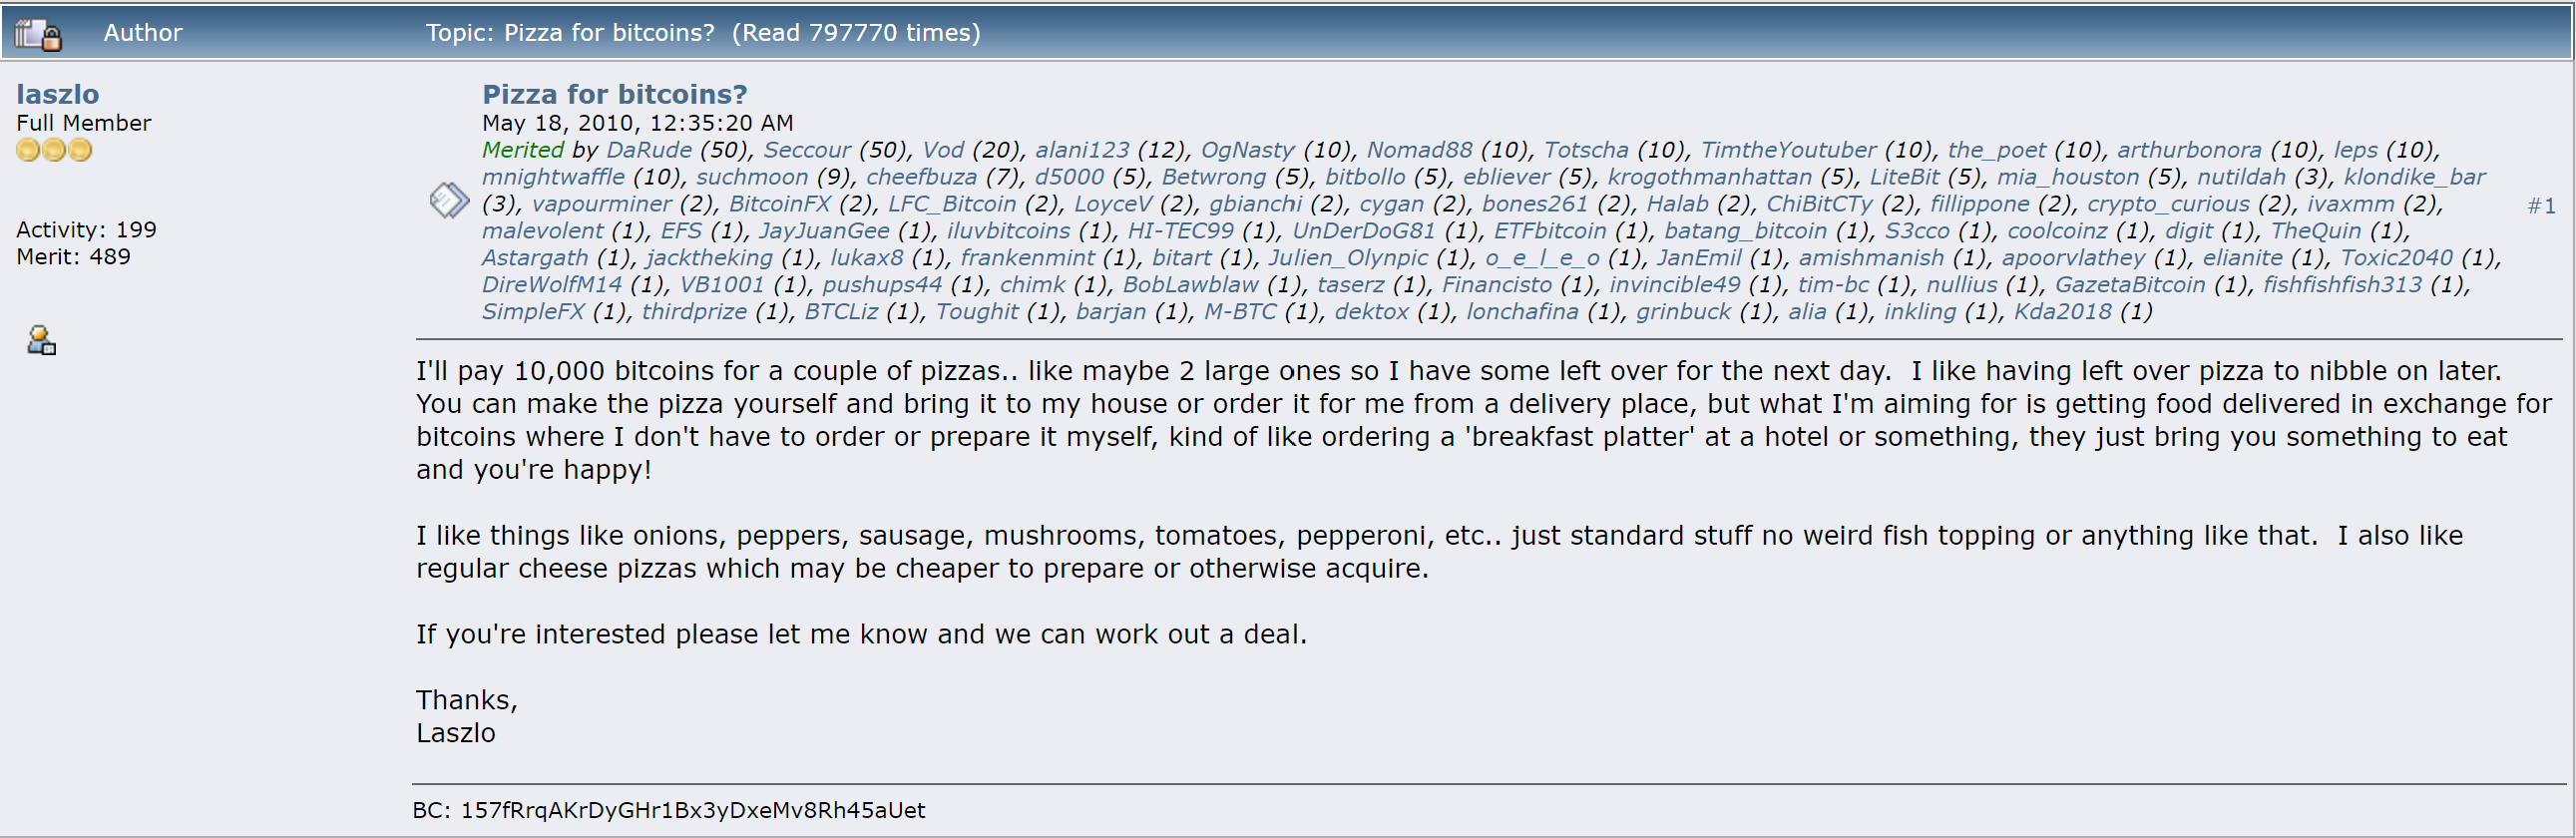
\includegraphics[scale=0.3]{../assets/images/pizza_blogpost}	
	\caption*{\href{https://bitcointalk.org/index.php?topic=137.0}{\link bitcointalk.org}}
	\end{figure}
\end{frame}
%%%

%%%
\begin{frame}{From Public Key to Bitcoin Address}
\vspace{-0.5em}
\begin{figure}
	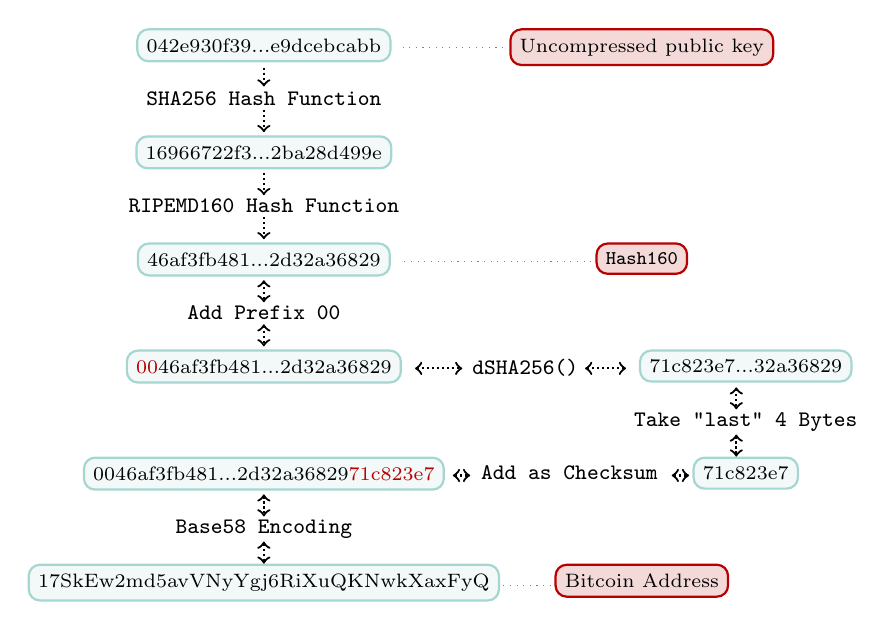
\begin{tikzpicture}[domain=-8:8,scale=0.4]

\draw[color=black] plot (0,8)    node[fill=highlight!15, thick, rounded corners=4pt,draw=highlight,below, rotate = 0] {{{\scriptsize 042e930f39...e9dcebcabb}}};

\draw[color = black] plot (12,8) node[fill=focus!15, thick, rounded corners=4pt, draw = focus, below, rotate = 0] {{{\scriptsize Uncompressed public key}}};

\draw[color=black] plot (0,6.3)   node[below, rotate = 0] {\texttt{\footnotesize{SHA256 Hash Function}}};

\draw[color=black] plot (0,4.6)    node[fill=highlight!15, thick, rounded corners=4pt,draw=highlight,below, rotate = 0] {{{\scriptsize 16966722f3...2ba28d499e}}};

\draw[color=black] plot (0,2.9)   node[below, rotate = 0] {\texttt{\footnotesize{RIPEMD160 Hash Function}}};

\draw[color=black] plot (0,1.2)    node[fill=highlight!15, thick, rounded corners=4pt,draw=highlight,below, rotate = 0] {{{\scriptsize 46af3fb481...2d32a36829}}};

\draw[color=black] plot (12,1.2)    node[fill=focus!15, thick, rounded corners=4pt,draw=focus,below, rotate = 0] {{{\scriptsize \texttt{Hash160}}}};

\draw[color=black] plot (0,-0.5)   node[below, rotate = 0] {\texttt{\footnotesize{Add Prefix 00}}};
 
\draw[color=black] plot (0,-2.2)    node[fill=highlight!15, thick, rounded corners=4pt,draw=highlight,below, rotate = 0] {{{\scriptsize \textcolor{focus}{00}46af3fb481...2d32a36829}}};

\draw[color=black] plot (8.3,-2.2)   node[below, rotate = 0] {\texttt{\footnotesize{dSHA256()}}};

\draw[color=black] plot (15.3,-2.2)    node[fill=highlight!15, thick, rounded corners=4pt,draw=highlight,below, rotate = 0] {{{\scriptsize 71c823e7...32a36829}}};

\draw[color=black] plot (15.3,-3.9)   node[below, rotate = 0] {{\footnotesize \texttt{Take "last" 4 Bytes}}};

\draw[color=black] plot (15.3,-5.6)    node[fill=highlight!15, thick, rounded corners=4pt,draw=highlight,below, rotate = 0] {\scriptsize{71c823e7}};

\draw[color=black] plot (9.7,-5.6)   node[below, rotate = 0] {\texttt{\footnotesize{Add as Checksum}}};

\draw[color=black] plot (0,-5.6)    node[fill=highlight!15, thick, rounded corners=4pt,draw=highlight,below, rotate = 0] {{{\scriptsize 0046af3fb481...2d32a36829\textcolor{focus}{71c823e7}}}};

\draw[color=black] plot (0,-7.3)   node[below, rotate = 0] {\texttt{\footnotesize{Base58 Encoding}}};

\draw[color=black] plot (0,-9)    node[fill=highlight!15, thick, rounded corners=4pt,draw=highlight,below, rotate = 0] {{{\scriptsize 17SkEw2md5avVNyYgj6RiXuQKNwkXaxFyQ}}};

\draw[color = black] plot (12,-9) node[fill=focus!15, thick, rounded corners=4pt, draw = focus, below, rotate = 0] {{{\scriptsize Bitcoin Address}}};

\draw[color=black, densely dotted,->, thick] (0,6.75) -- (0,6.15);
\draw[color=black, densely dotted,->, thick] (0,5.4) -- (0,4.7);
\draw[color=black, densely dotted,->, thick] (0,3.4) -- (0,2.7);
\draw[color=black, densely dotted,->, thick] (0,2) -- (0,1.3);
\draw[color=black, densely dotted,<->, thick] (0,0) -- (0,-0.7);
\draw[color=black, densely dotted,<->, thick] (0,-1.4) -- (-0,-2.1);

\draw[color=black, densely dotted,<->, thick] (4.8,-2.8) -- (6.3,-2.8);
\draw[color=black, densely dotted,<->, thick] (10.2,-2.8) -- (11.5,-2.8);

\draw[color=black, densely dotted,<->, thick] (15,-3.4) -- (15,-4.1);
\draw[color=black, densely dotted,<->, thick] (15,-4.9) -- (15,-5.6);

\draw[color=black, densely dotted,<->, thick] (6,-6.2) -- (6.55,-6.2);
\draw[color=black, densely dotted,<->, thick] (12.95,-6.2) -- (13.5,-6.2);

\draw[color=black, densely dotted,<->, thick] (0,-6.8) -- (0,-7.5);
\draw[color=black, densely dotted,<->, thick] (0,-8.3) -- (0,-9);

\draw[dotted, color = black!50] (7.6, 7.4) -- (4.3, 7.4);
\draw[dotted, color = black!50] (10.4, 0.6) -- (4.3, 0.6);
\draw[dotted, color = black!50] (7.6, -9.7) -- (9.1, -9.7);
\end{tikzpicture}
\end{figure}
\vspace{-1em}
\scriptsize
\href{https://github.com/cifunibas/Bitcoin-Blockchain-Cryptoassets/blob/main/assets/scripts/bitcoin_address.py}{\link Python script for each step} \\
\end{frame}
%%%

%%%
\begin{frame}{Raw Transaction Data}
	\begin{itemize}
		\item The transaction uses 131 inputs.
		\item The complete raw transaction data is very long.
		\item Let's focus on the unlocking condition and differences to P2PK.
	\end{itemize}
\end{frame}
%%%

%%%
\begin{frame}{Raw Transaction Data (Output)}
\begin{scriptsize}
\texttt{\textcolor{black!30}{01000000830d2e8f94c33a10f3834554cc1f1469e069f0fcf31a47309d42a9d00f4ba5
7d86000000008c493046022100bc57dc26f46fecc1da03272cb2298d8a08b22d865541
f5b3a3e862cc87da4b47022100ce1fc72771d164d608b15065832542a0e9040cfdf288
62c5175c81fcb0e0b65501410434417dd8d89deaf0f6481c2c160d6de0921624ef7b95
6f38eef9ed4a64e36877be84b77cdee5a8d92b7d93694f89c3011bf1cbdf4fd7d8ca13
b58a7bb4ab0804ffffffff}\alert<1>{...}{\alert<2>{01}\alert<3>{0010a5d4e8000000}\alert<4>{19}\alert<5>{76}\alert<6>{a9}\alert<7>{14}\alert<8>{46af3fb481837fadbb4
21727f9959c2d32a36829}\alert<9>{88}\alert<10>{ac}}\textcolor{black!30}{00000000}}
\end{scriptsize}
\vspace{1em}
	\scriptsize \\
	\textbf{The output consists of:}\\
	\begin{columns}
	\column{0.5\textwidth}
	\begin{itemize}
		\item \alert<2>{1 output: \texttt{01}}
		\item \alert<3>{10,000 BTC: \texttt{0010a5d4e8000000}}
		\item \alert<4>{26 byte long \texttt{scriptPubKey}: \texttt{19}}
		\item \textcolor{black!50}{\alert<5>{\texttt{OP\_DUP}: \texttt{76}}}
		\item \textcolor{black!50}{\alert<6>{\texttt{OP\_HASH160}: \texttt{a9}}}
	\end{itemize}
	\column{0.5\textwidth}
	\begin{itemize}
		\item \alert<7>{20 byte long Public Key Hash: \texttt{14}}
		\item \alert<8>{\texttt{Hash160}:\\
		\texttt{46af3fb481837fadbb42\\1727f9959c2d32a36829}}
		\item \textcolor{black!50}{\alert<9>{\texttt{OP\_EQUALVERIFY}: \texttt{88}}}
		\item \textcolor{black!50}{\alert<10>{\texttt{OP\_CHECKSIG}: \texttt{ac}}}
	\end{itemize}
	\end{columns}
	\vspace{1em}
	\normalsize
	\uncover<11->{$\rightarrow$ You can spend the 10,000 BTC if you know the private key to the public key which hashes to \texttt{46af...6829}}\\
\end{frame}
%%%

%%%
\begin{frame}{Raw Transaction Data (Inputs)}
\begin{scriptsize}
\texttt{\textcolor{black!30}{01000000}{\alert<2>{83}\alert<3>{0d2e8f94c33a10f3834554cc1f1469e069f0fcf31a47309d42a9d00f4ba5
7d86}\alert<4>{00000000}}\textcolor{black!30}{8c493046022100bc57dc26f46fecc1da03272cb2298d8a08b22d865541
f5b3a3e862cc87da4b47022100ce1fc72771d164d608b15065832542a0e9040cfdf288
62c5175c81fcb0e0b65501410434417dd8d89deaf0f6481c2c160d6de0921624ef7b95
6f38eef9ed4a64e36877be84b77cdee5a8d92b7d93694f89c3011bf1cbdf4fd7d8ca13
b58a7bb4ab0804ffffffff...010010a5d4e80000001976a91446af3fb481837fadbb4
21727f9959c2d32a3682988ac00000000}}
\end{scriptsize}
\vspace{1em}
\scriptsize \\
\textbf{The inputs consist of:}\\
\begin{itemize}
	\item \alert<2>{131 inputs: \texttt{83}}
	\item \alert<3>{Previous transaction in reverse byte order: \texttt{0d2e8f94c33a10f3834554cc1f1469e069f0fcf31a47309d42a9d00f4ba57d86}}
	\item \alert<4>{Index of the output within the previous transaction as little-endian integer: \texttt{00000000}}
	\item ...
\end{itemize}
\end{frame}
%%%

%%%
\begin{frame}{Raw Transaction Data (Signature)}
\begin{scriptsize}
\texttt{\textcolor{black!30}{01000000830d2e8f94c33a10f3834554cc1f1469e069f0fcf31a47309d42a9d00f4ba5
7d8600000000}{\alert<2>{8c}\alert<3>{49}\alert<4>{30}\alert<5>{46}\alert<6>{02}\alert<7>{21}\alert<8>{00bc57dc26f46fecc1da03272cb2298d8a08b22d865541
f5b3a3e862cc87da4b47}\alert<9>{02}\alert<10>{21}\alert<11>{00ce1fc72771d164d608b15065832542a0e9040cfdf288
62c5175c81fcb0e0b655}\alert<12>{01}\alert<13>{41}\alert<14>{04}\alert<15>{34417dd8d89deaf0f6481c2c160d6de0921624ef7b95
6f38eef9ed4a64e36877be84b77cdee5a8d92b7d93694f89c3011bf1cbdf4fd7d8ca13
b58a7bb4ab0804}}\textcolor{black!30}{ffffffff...010010a5d4e80000001976a91446af3fb481837fadbb4
21727f9959c2d32a3682988ac00000000}}
\end{scriptsize}
\vspace{1em}
\scriptsize \\
\textbf{The signature consists of:}\\
\begin{columns}[T]
\column{0.5\textwidth}
\begin{itemize}
	\item \alert<2>{140 byte long \texttt{scriptSig}: \texttt{8c}}
	\item \alert<3>{73 byte long signature: \texttt{49}}
	\item \alert<4>{DER sequence follows: \texttt{30}}
	\item \alert<5>{70 bytes long: \texttt{46}}
	\item \alert<6>{An integer follows: \texttt{02}}
	\item \alert<7>{The integer is 33 bytes long: \texttt{21}}
	\item \alert<8>{$r$ from the ECDSA signature: 	\texttt{00bc57dc26f46fecc1da03272cb2298d8\\
	a08b22d865541f5b3a3e862cc87da4b47}}
	\item \alert<9>{An integer follows: \texttt{02}}
	\item \alert<10>{The integer is 33 bytes long: \texttt{21}}
\end{itemize}
\column{0.5\textwidth}
\begin{itemize}
	\item \alert<11>{$s$ from the ECDSA signature: \texttt{00ce1fc72771d164d608b15065832542a\\
	0e9040cfdf28862c5175c81fcb0e0b655}}
	\item \alert<12>{\texttt{SIGHASH\_ALL}: \texttt{01}}
	\item \alert<13>{65 byte long public key: \texttt{41}}
	\item \alert<14>{Uncompressed public key: \texttt{04}}
	\item \alert<15>{Public key: \texttt{34417dd8d89deaf0f6481c2c160d6de0\\
	921624ef7b956f38eef9ed4a64e36877\\
	be84b77cdee5a8d92b7d93694f89c301\\
	1bf1cbdf4fd7d8ca13b58a7bb4ab0804}}
\end{itemize}
\end{columns}
\end{frame}
%%%

%%%
\begin{frame}{Raw Transaction Data (Additional Data)}
\begin{scriptsize}
\texttt{\alert<2>{01000000}\textcolor{black!30}{830d2e8f94c33a10f3834554cc1f1469e069f0fcf31a47309d42a9d00f4ba5
7d86000000008c493046022100bc57dc26f46fecc1da03272cb2298d8a08b22d865541
f5b3a3e862cc87da4b47022100ce1fc72771d164d608b15065832542a0e9040cfdf288
62c5175c81fcb0e0b65501410434417dd8d89deaf0f6481c2c160d6de0921624ef7b95
6f38eef9ed4a64e36877be84b77cdee5a8d92b7d93694f89c3011bf1cbdf4fd7d8ca13
b58a7bb4ab0804}\alert<3>{ffffffff}...\textcolor{black!30}{010010a5d4e80000001976a91446af3fb481837fadbb4
21727f9959c2d32a3682988ac}\alert<4>{00000000}}
\end{scriptsize}
\vspace{1em}
\scriptsize \\
\uncover<1->{\textbf{Additional data used in raw transactions:}}\\
\begin{itemize}
	\item \alert<2>{Version as little-endian integer: \texttt{01000000}}
	\item \alert<3>{Sequence number (deprecated): \texttt{ffffffff}}
	\item \alert<4>{Timelock: \texttt{00000000}}
\end{itemize}
\end{frame}
%%%


%%%
\begin{frame}{Bitcoin Script}
\begin{columns}
\column{0.5\textwidth}
\begin{figure}
	\begin{tikzpicture}[scale=1, every node/.style={scale=1.2}]  %,domain=0:8

%Stack
\draw[very thick] (-0.1,0) -- (4.1,0);
\draw[very thick] (-0.1,0) -- (-0.1,4);
\draw[very thick] (4.1,0) -- (4.1,4);
\draw (2,-0.5) node[below] {\texttt{Stack}};

%Boxes
\only<1-14>{
\draw[color=black] plot (2,0.7)   node[minimum width=2.7cm,fill=highlight!15, thick, draw=highlight,below, rotate = 0] {\texttt{483045...ee0e01}};
  }
  
\only<1,2,5-14>{
\draw[color=black] plot (2,1.4)   node[minimum width=2.7cm,fill=highlight!15, thick,  draw=highlight,below, rotate = 0] {\texttt{042e93...ebcabb}};
}

\only<5,6>{
\draw[color=black] plot (2,2.1)   node[minimum width=2.7cm, fill=highlight!15, thick,  draw=highlight,below, rotate = 0] {\texttt{042e93...ebcabb}};
}

%OP Codes
\only<2,3>{
\draw[color=black] plot (6,4.8)   node[minimum width=3.1cm ,fill=black!15, thick,  draw=black,below, rotate = 0] {\texttt{76}};
}

\only<6,7>{
\draw[color=black] plot (6,4.8)   node[minimum width=3.1cm ,fill=black!15, thick,  draw=black,below, rotate = 0] {\texttt{a9}};
}

\only<11,12>{
\draw[color=black] plot (6,4.8)   node[minimum width=3.1cm, fill=black!15, thick,  draw=black,below, rotate = 0] {\texttt{88}};
}

\only<14,15>{
\draw[color=black] plot (6,4.8)   node[minimum width=3.1cm, fill=black!15, thick,  draw=black,below, rotate = 0] {\texttt{ac}};
}

%Boxes 2
\only<3,4,7>{
\draw[color=black] plot (2,4.8)   node[minimum width=2.7cm,fill=highlight!15, thick,  draw=highlight,below, rotate = 0] {\texttt{042e93...ebcabb}};
}

\only<4>{
\draw[color=black] plot (2,4.1)   node[minimum width=2.7cm,fill=highlight!15, thick,  draw=highlight,below, rotate = 0] {\texttt{042e93...ebcabb}};
}

\only<8,12>{
\draw[color=black] plot (2,4.8)   node[minimum width=2.7cm,fill=highlight!15, thick,  draw=highlight,below, rotate = 0] {\texttt{46af3f...a36829}};
}

\only<9,10,11>{
\draw[color=black] plot (2,2.1)   node[minimum width=2.7cm,fill=highlight!15, thick,  draw=highlight,below, rotate = 0] {\texttt{46af3f...a36829}};
}

\only<10,11>{
\draw[color=black] plot (2,2.8)   node[minimum width=2.7cm,fill=focus!15, thick,  draw=focus,below, rotate = 0] {\texttt{46af3f...a36829}};
}

\only<12>{
\draw[color=black] plot (2,4.8)   node[minimum width=2.7cm,fill=focus!15, thick,  draw=focus,below, rotate = 0] {\texttt{46af3f...a36829}};
}

\only<12>{
\draw[color=black] plot (2,4.1)   node[minimum width=2.7cm,fill=highlight!15, thick,  draw=highlight,below, rotate = 0] {\texttt{46af3f...a36829}};
}

\only<15>{
\draw[color=black] plot (2,4.8)   node[minimum width=2.7cm,fill=highlight!15, thick,  draw=highlight,below, rotate = 0] {\texttt{042e93...ebcabb}};
}

\only<15>{
\draw[color=black] plot (2,4.1)   node[minimum width=2.7cm,fill=highlight!15, thick,  draw=highlight,below, rotate = 0] {\texttt{483045...ee0e01}};
}

\only<16>{
\draw[color=black] plot (2,0.7)   node[minimum width=3.3cm,fill=highlight!15, thick,  draw=highlight,below, rotate = 0] {\texttt{1}};
}

%Dummy
\only<1,4,5,8,9,10,13,16>{
\draw[color=white] plot (6,4.8)   node[minimum width=3.1cm,fill=white, thick,  draw=white,below, rotate = 0] {\texttt{OP\_HASH160}};
}

\end{tikzpicture}
\end{figure}
\column{0.5\textwidth}
\begin{enumerate}
\item<1-> \texttt{<sig>} and \texttt{<pubKey>}
\item<2-> \texttt{OP\_DUP}
\item<6-> \texttt{OP\_HASH160}
\item<10-> \texttt{pubKeyHash}
\item<11-> \texttt{OP\_EQUALVERIFY}
\item<14-> \texttt{OP\_CHECKSIG}
\end{enumerate}
\end{columns}
\end{frame}
%%%

\end{document}